\documentclass{article}

\input{../../../preambule}

\newtheorem{theorem}{Théorème}[subsection]

\title{Pr\'esentation d'un article : \\ On shape optimization of optical waveguides using inverse problem techniques\\\small{Thomas Felici \& Heinz W Engl}}
\author{Alexandre \bsc{Vieira}}
\date{\today}

\hypersetup{colorlinks=true, urlcolor=bleu, linkcolor=red}

\begin{document}

\maketitle
\tableofcontents

\newpage

\section*{Introduction}
Les guides d'ondes optiques sont à la base de l'optoéléctronique, ie les composants éléctroniques interagissant avec de la lumière, et de l'industrie des télécommunications. L'exemple le plus connu est bien évidemment la fibre optique, mais il existe également d'autres exemples tout aussi important, comme les composants optiques qui manipulent, filtrent et dispatchent des signaux entrants. Ces composants sont souvent de l'ordre du quart de nanomètre, ce qui représente bien sûr un avantage en poids et en volume, et qui permettent de remplir des fonctions que ne peuvent pas faire des objets plus classiques. Le développement de cette technologie repose de plus en plus sur des modèles mathématiques de paire avec des simulations numériques pour la prédiction du comportement de ces appareils, ainsi que la production d'un appareil 'optimal', ce qui repose bien souvent sur des modèles reposant sur des EDP.\\
Les adaptateurs de mode intégrés, aussi appelés "taper" en anglais, est un guide d'onde dont la section varie sur sa longueur, utilisés comme des sortes d'entonnoir. Il est bien connu que si le taper est assez long, la lumière sera transmise sans perte d'énergie. Mais plus la longueur est courte, plus le faisceau perd en énergie. Le but de ce papier était donc de trouver une formulation pour minimiser la perte d'énergie pour une longueur donnée.\\
Dans un premier temps, l'article met en place un premier problème direct pour la propagation d'une onde éléctromagnétique à traver un guide d'onde, puis il définit le problème d'optimisation. Comme on le vera, on peut ensuite dériver de ce modèle une formulation pour les modes, et établir des équations d'évolution pour l'excitation des modes dans le taper. Une problème d'optimisation en dimension finie basée sur une discrétisation sortira enfin de tout cela. \\
Des exemples numériques basés sur cette méthode montre que si la discrétisation devient trop fine, la convergence ralentit et la solution devient de plus en plus instable. Le problème vient du fait qur le problème d'optimisation est mal posé. L'article présente donc une méthode pour maximiser l'énergie résultante basée sur un problème inverse non linéaire, ainsi que des résultats numériques coroborant leur idée. 

\section{Formulation du problème direct en 2D}
Les équations homogènes de Maxwell dans un milieu continu avec la permitivité linéaire $\varepsilon$ et la perméabilité magnétique $\mu_0$ sont :
\begin{equation}\label{MaxEq}
\begin{array}{c c c}
	\nabla\wedge H&=& \varepsilon\dot{E}\\
	\nabla\wedge E&=& -\mu_0\dot{H}\\
	\nabla\bullet(\varepsilon E)&=&\nabla\bullet H=0
\end{array}
\end{equation}
On se concentre uniquement sur le cas 2D. On assume donc que $E$ et $H$ sont indépendants de $y$. Si on assume une dépendance périodique en temps $e^{-i\omega t}$ et qu'on note $E=(E_x,E_y,E_z)$ et $H=(H_x,H_y,H_z)$ les composantes spatiales de la solution, on a une solution avec $H_y=E_x=E_z=0$ - le champ TE (transverse electric) - vérifiant :
\begin{equation} \label{eq2}
\begin{array}{c c c}
	\frac{\partial H_x}{\partial z} - \frac{\partial H_z}{\partial x}&=&-i\omega\varepsilon E_y\\
	\frac{\partial E_y}{\partial z}&=&-i\omega\mu_0H_x\\
	\frac{\partial E_y}{\partial x}&=&i\omega\mu_0  H_z
\end{array}
\end{equation}

En redérivant les deux dernières équations de (\ref{eq2}) par rapport à respectivement $z$ et $x$ et en réintroduisant le résultat dans la première équation, on obtient l'équation d'Helmholtz pour $E_y$ :
\[ \Delta E_y + k^2n^2E_y = 0 \text{ avec } \omega\sqrt{\mu_0\varepsilon_0}=k \text{ et } n^2=\frac{\varepsilon}{\varepsilon_0} \]
où $\varepsilon_0$ désigne la permitivité du vide.

On remarque également qu'on obtient une solution avec $E_y=H_x=H_z=0$ -le champ magnétique transverse ('TM') - donnant une équation légèrement modifiée :
	\[-\Delta H_y+k^2n^2H_y=0\]

Cependant, l'analyse ne se poursuivra qu'avec les modes du champ TE.

\bigskip
\begin{figure}[!h]
	\centering
	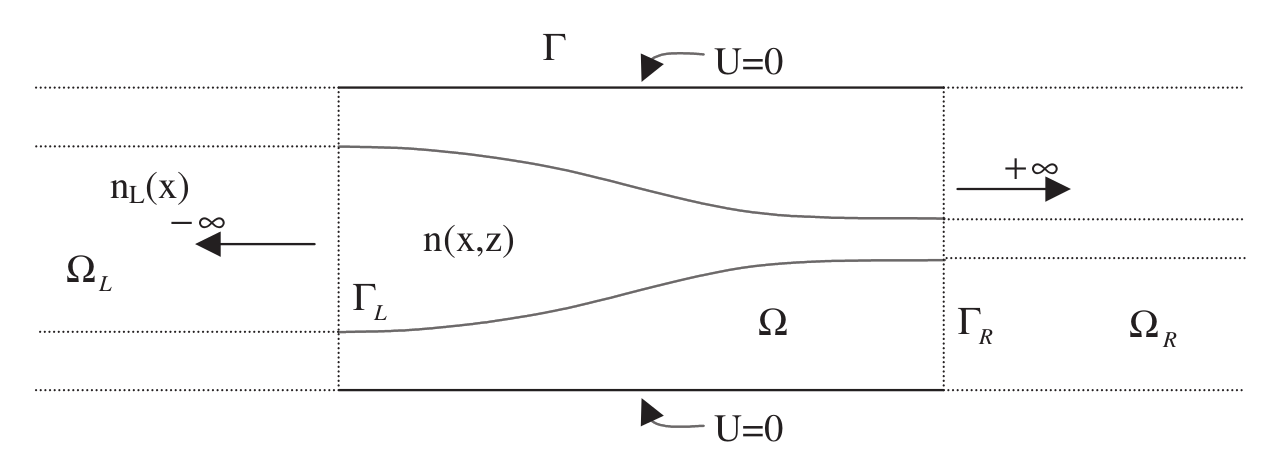
\includegraphics[scale=0.35]{images/waveguide-Taper.png}
	\caption{Profil du taper}
	\label{fig:Profil}
\end{figure}
Nous allons maintenant formuler le problème de propagation de l'onde dans un guide d'onde générique $\Omega$ en notant la frontière $\Gamma\cup\Gamma_R\cup\Gamma_L$ (voir la figure \ref{fig:Profil}).\\
À présent, pour plus de commodité, $E_y$ sera noté $U$. Sur le bord $\Gamma$, nous prenons des conditions de Dirichlet ($U=0$). Physiquement, cela signifie que le champ est réfléchi vers $\Omega$. En pratique, cela n'est pas un problème si on cherche des solutions de champs guidés, car ils sont par définition limités au guide d'onde et décroissent exponentiellement en dehors (ce qui sera discuté plus en détail ultérieurement). On réécrit donc les équations :
\begin{eqnarray}
	\label{eq3} \Delta U + n^2U&=&0 \text{ pour } (x,z)\in\Omega\\
	\label{eq4} \restriction{U}{\Gamma}&=&0
\end{eqnarray}
où on a posé $k=1$. Cela n'est rien d'autre qu'une normalisation de l'équation : on pose simplement $x'=kx$ et $z'=kz$. Ainsi : 
	\[(\partial^2_x+\partial^2_z)U(x',z')=k^2 (\partial^2_{x'}+\partial^2_{z'})U(x',z')=k^2\Delta U(x',z')\]
D'où :
	\[k^2\Delta U + n^2k^2 U =0\]
On obtient l'équation précédente en simplifiant par $k^2$.

\bigskip
Nous avons besoin à présent de conditions à $\pm\infty$. Nous prenons comme hypothèse que nous avons un champ entrant venant de $-\infty$. Ce champ $U_I$ satisfait également (\ref{eq3}), (\ref{eq4}) dans $\Omega_L$. Nous devons retrouver le fait que le champ diffusé $U-U_I$ voyage vers l'extérieur des deux côtés du guide d'onde. Nous allons faire cela en terme de modes propres dans $\Omega_L$ et $\Omega_R$, ce qui amène donc à considérer un problème spectral dans ces régions.\\
Dans $\Omega_L$, on prend une dépendance périodique par rapport à $z$ : $U(x,z)=\tilde{U}(x)e^{i\beta z}$. En réinjectant cela dans (\ref{eq3}), on obtient :
\begin{equation}\label{eq5} \frac{d^2\tilde{U}}{dx^2} + (n^2-\beta^2)\tilde{U}=0 \text{ pour un } z \text{ fixé avec } \tilde{U}(x_{min})=\tilde{U}(x_{max})=0 \end{equation}

Les conditions de Dirichlet (\ref{eq4}) nous assure que nous avons en ensemble de valeurs propres discrètes $\{(\tilde{U}_k,\pm\beta_k):k\in\mathbb{N}^*\}$. On a donc :
\begin{equation}\label{eq6} U(x,z)=\sum_{k=1}^\infty \left(C_ke^{i\beta_k z}+C_{-k}e^{-i\beta_k z}\right) \tilde{U}_k(x) \text{ dans } \Omega_L \end{equation}

Notons que le raisonnement tient toujours dans $\Omega_R$ et donne un résultat similaire.\\
Dans (\ref{eq6}), on pose $\beta_k>0$ si $\beta_k$ est réel, $\beta_k=i|\beta_k|$ si $\beta_k$ est imaginaire. Ainsi, les coefficients $C_k$ et $C_{-k}$ représentent respectivement le voyage vers la droite et vers la gauche de l'onde.\\
De plus, on remarque que l'opérateur utilisé dans (\ref{eq3}) est auto-adjoint pour le produit scalaire $\langle a,b\rangle = \int_{x_{min}}^{x_{max}} a(x)b(x)dx$. En effet :
\begin{eqnarray*}
\left\langle (\Delta +n^2 Id)u,v\right\rangle&=&\langle \Delta u,v\rangle + \langle n^2u,v\rangle \\
					&=&\int_{x_{min}}^{x_{max}} \Delta u(x) v(x) dx + \langle u,n^2 v \rangle \\
					&=&-\int_{x_{min}}^{x_{max}} \nabla u(x). \nabla v(x) dx + \underbrace{\left[\nabla u(x).n v(x)\right]_{x_{min}}^{x_{max}}}_{=0 \text{ dû au conditions de Dirichlet}}+ \langle u,n^2 v \rangle \\
					&=& \int_{x_{min}}^{x_{max}} u(x) \Delta v(x) dx - \underbrace{\left[\nabla v(x).n u(x)\right]_{x_{min}}^{x_{max}}}_{=0} + \langle u,n^2 v \rangle \\
					&=& \left\langle u,(\Delta +n^2 Id)v\right\rangle
\end{eqnarray*}

Cela assure ainsi que les modes propres sont orthogonaux relativement à ce produit scalaire. De plus, si on normalise les normes :
\begin{equation} \label{eq7} \langle \tilde{U}_k,\tilde{U}_k\rangle = \frac{1}{\beta_k} \end{equation}
la puissance transmise dans chaque mode propre $k$ est donné par $|C_k|^2$.\\
Étant donné cette normalisation, une onde sortante $U_L$ (vers $-\infty$) est donnée en posant $C_k=0$ pour tout $k>0$. Ainsi :
\begin{eqnarray*}
\beta_k\langle U_L,\tilde{U}_k\rangle &=&\beta_k\sum_{j=1}^\infty C_{-j}e^{-i\beta_j z}\langle \tilde{U}_j,\tilde{U}_k \rangle \\
				      &=&\beta_k C_{-k} e^{-i\beta_k z} \frac{1}{\beta_k}\\
				      &=&C_{-k} e^{-i\beta_k z}
\end{eqnarray*}

De même, une onde entrante $U_I$ est donnée en fixant $C_{-k}=0$ pour tout $k>0$ et $C_k$ est donné par \[C_ke^{i\beta_k z}=\beta_k\langle U_I,\tilde{U}_k\rangle\]
Enfin, on différencie (\ref{eq6}) pour $U_L$ et $U_I$ pour obtenir les conditions au bord sur les côtés. On obtient ainsi :
\[\frac{\partial U_L}{\partial z} =\sum_{k=1}^\infty -i \beta_k C_{-k} e^{-i\beta_k z} \tilde{U}_k(x)\]
\begin{equation} \label{eq8} 
\frac{\partial U_L}{\partial z}= -i \sum_{k=1}^\infty \beta_k^2 \langle U_L,\tilde{U}_k\rangle \tilde{U}_k(x) \text{ dans }\Omega_L\text{ - condition pour les ondes partant vers }-\infty
\end{equation}
De même : 
\begin{equation} \label{eq9} 
\frac{\partial U_I}{\partial z}= -i \sum_{k=1}^\infty \beta_k^2 \langle U_I,\tilde{U}_k\rangle \tilde{U}_k(x) \text{ dans }\Omega_L\text{ - condition pour les ondes venant de }-\infty
\end{equation}

Puisque $U=U_I+U_L$, en replaçant $U_L$ dans (\ref{eq8}) et en utilisant (\ref{eq9}), on obtient : 
	\[\frac{\partial U}{\partial z}=-i\sum_{k=1}^\infty {\beta_k^{(L)}}^2\left\langle U,\tilde{U}^{(L)}_k\right\rangle \tilde{U}^{(L)}_k + 2i\sum_{k=1}^\infty {\beta_k^{(L)}}^2 \left\langle U_I,\tilde{U}_k^{(L)}\right\rangle\tilde{U}^{(L)}_k \]
En surmontant le tout de l'exposant $(L)$ pour indiquer que le tout vient de la gauche, ie de $-\infty$.\\
De même, pour les ondes se propageant vers $+\infty$, et en supposant qu'il n'y a aucune onde venant de là, on obtient :
\[\frac{\partial U}{\partial z}=i\sum_{k=1}^\infty {\beta_k^{(R)}}^2 \left\langle U,\tilde{U}_k^{(R)} \right\rangle \tilde{U}_k^{(R)} \text{ dans } \Omega_R \text{ - condition pour les ondes allant vers }+\infty\]
Le problème complet est donc : trouver $U(x,z)$ tel que : 
\begin{equation} \label{eq10}
\left\{\begin{array}{r c l r}
	\Delta U + n^2U&=&0 &\text{pour } (x,z)\in\Omega\\
	\restriction{U}{\Gamma}&=&0 &\text{(murs réfléchissants)}\\
	\frac{\partial U}{\partial z}+i\sum_{k=1}^\infty {\beta_k^{(L)}}^2\left\langle U,\tilde{U}^{(L)}_k\right\rangle \tilde{U}^{(L)}_k &=& 2i\sum_{k=1}^\infty {\beta_k^{(L)}}^2 \left\langle U_I,\tilde{U}_k^{(L)}\right\rangle\tilde{U}^{(L)}_k &\text{sur }\Gamma_L\\
	\frac{\partial U}{\partial z}-i\sum_{k=1}^\infty {\beta_k^{(R)}}^2 \left\langle U,\tilde{U}_k^{(R)} \right\rangle \tilde{U}_k^{(R)}&=&0 &\text{sur } \Gamma_R
\end{array}\right.
\end{equation}
où $\{(\tilde{U}_k^{(L)},\pm\beta_k^{(L)}):k\in\mathbb{N}^*\}$, $\{(\tilde{U}_k^{(R)},\pm\beta_k^{(R)}):k\in\mathbb{N}^*\}$ sont les modes propres dans $\Omega_L$, $\Omega_R$ respectivement.

\section{Formulation du problème d'optimsation}
En général, nous nous interessons à la forme optimale du taper (ou la distribution des indices de refraction) qui dans un sens maximise la puissance transférée entre l'entrée et la sortie du guide d'onde.\\
Souvent, pour des raisons pratiques, on suppose que l'onde en entrée est une excitation de l'élément propre fondamental (indicé donc par $1$), et on s'intéresse à la puissance restante dans l'élément propre fondamental $\tilde{U}^{(R)}_1$ de l'onde de sortie (on assume bien évidemment que les deux ondes admettent au moins un mode guidé). Dans la décomposition spectral (\ref{eq6}), l'énergie restante correspond au coefficient $|C_1|^2$. Cela est donné par :
\begin{equation}\label{eq11} P(n^2)=\beta_1^2|\langle U,\tilde{U}_1^{(R)}\rangle|^2=\beta_1^2\left|\int_{x\in\Gamma_R} U(x,z_R)\tilde{U}_1^{(R)}(x)dx\right|^2\end{equation}
Intuitivement (et cela se vérifie, comme montré dans \cite{Snyd}), la puissance transférée est maximale (ie $P=1$) quand la longueur du taper tend vers l'infini. Il est donc évident qu'on doit imposer une contrainte supplémentaire sur la longueur finie du taper.

\section{Solution du problème direct}
\subsection{Recherche d'une représentation locale}
À cause des conditions aux bords que nous avons imposé, le système (\ref{eq10}) est en général résolu en utilisant une décomposition spectrale.\\
On définit $L_t(U)=\frac{\partial^2U}{\partial x^2}+n^2(x,z)U$ l'opérateur 1D de Helmholtz.\\
Soit $\Omega_z$ la section de la région au point $z$. On définit la base locale $\{(U_k,\beta_k);k\geq 1\}$ à chaque position $z$ par : 
\begin{equation} \label{eq13}
	\begin{array}{c c c c}
		L_t(U_k)&=&\beta_k^2U_k &\text{dans } \Omega_z\\
		\restriction{U_k}{\partial\Omega_z}&=&0
	\end{array}
\end{equation}
Cela est analogue à (\ref{eq5}), donc nous parlerons des solutions $U_k$ comme les fonctions propres locales. Le caractère auto-adjoint de l'opérateur $L_t$ (comme on l'a prouvé précédemment) assure que les $(U_k)$ forment une base orthogonale pour les fonctions $f\in\mathscr{C}(\Omega_z)$ avec $\restriction{f}{\partial\Omega_z}=0$. Ainsi, toute fonction $U$ définie dans une région $\Omega$ avec $\restriction{U}{\partial\Omega_z}=0$ peut être exprimé comme l'unique décomposition $U=\sum_{k=1}^\infty c_k(z)U_k$ où les coefficients (uniques) $c_k$ dépendent exclusivement de $z$.\\
On s'intéresse maintenant à une formulation qui donne une représentation locale du champ éléctromagnétique en terme de propagation vers $-\infty$ ou $+\infty$ des modes du champ EM.
On choisit donc le développement de notre fonction $U$ solution de (\ref{eq10}) de la forme :
\begin{equation}\label{eq14}
\begin{array}{c c l}
U&=&\sum_{k=1}^\infty (a_k+a_{-k})U_k\\
\frac{\partial U}{\partial z}&=&\sum_{k=1}^\infty (a_k-a_{-k})i\beta_kU_k
\end{array}
\end{equation}
Ce choix de coefficients nous assure que les $a_k$, $a_{-k}$ correspondent aux champs se propageant vers $+\infty$ ou $-\infty$. On réutilise la normalisation (\ref{eq7}) pour les fonctions propres $U_k$ définies par (\ref{eq13}) :
\begin{equation}\label{eq15}
	\int_{\Omega_z} U_k^2ds=\frac{1}{\beta_k}
\end{equation}
Cela assure que la puissance contenue dans le $k^{ieme}$ mode de l'onde se propageant de chaque côté est obtenu par $|a_k|^2$ ou $|a_{-k}|^2$ (voir \cite{Snyd} pour plus de détail).\\
On remarque en particulier que l'énergie contenue dans l'état fondamental à la sortie du guide d'onde est maintenant 
\begin{equation}\label{eq16} P(n^2)=|a_1|^2\end{equation}
En référence à l'expression (\ref{eq11}).\\
En utilisant le fait que la dérivée par rapport à $z$ de $U$ en (\ref{eq14}) doit être identique à la seconde ligne de (\ref{eq14}), et en substituant (\ref{eq14}) dans (\ref{eq3}), on en déduit que les $a_k$ doivent vérifier le système d'EDO suivant :
\begin{equation} \label{eq17}
\dot{a}_k(z)-i\beta_ka_k(z)=\sum_{j\neq k,0} r_{kj}(z)a_j(z),\ k\neq 0
\end{equation}
avec $\beta_{-k}=-\beta_k$ et \[r_{kj}(z)=\frac{\int_{\Omega_z} \frac{\partial n^2}{\partial z} U_kU_j ds}{2(\beta_k-\beta_j)}\]
pour tout $j\neq k$, $j,k\neq 0$\\
\subsection{Démonstration}
Précisons tout d'abord que nous allons noter pour plus de commodité $U_{-k}=-U_k$. Pour démontrer (\ref{eq17}), on différencie (\ref{eq14}) et on l'identifie à la seconde ligne, on obtient que $a_k$ vérifie :
	\[\sum_{k\neq 0} \dot{a}_kU_k + \sum_{k\neq 0} a_k\frac{\partial U_k}{\partial z} = \sum_{k\neq 0} a_ki\beta_k U_k\]
Par orthogonalité des $U_k$, on projette cette équation sur chaque $U_i$, et cela mène à :
\begin{equation}\label{eq29}
	\dot{a}_k+\dot{a}_{-k}=(a_k-a_{-k})i\beta_k-\sum_{j\neq 0} a_j p_{jk}\ \forall k\neq 0
\end{equation}
où $p_{jk}=\beta_{|k|}\int_{\Omega_z} \frac{\partial U_j}{\partial z}U_k dx$ ne sont pas moins que les coefficients du développement de $\frac{\partial U_j}{\partial z}$ dans la base des $(U_k)$.\\
La première expression de (\ref{eq3}) peut être réécrite \[\frac{\partial^2 U}{\partial z^2}+L_t(U)=0\]
Et donc, en utilisant (\ref{eq14}) :
\[\frac{\partial}{\partial z} \left( \sum_{k\neq 0} a_ki\beta_kU_k\right)+L_t\left(\sum_{k\neq 0} a_kU_k\right) = 0\]
comme $L_t$ est linéaire :
\begin{eqnarray*}
\Rightarrow& \frac{\partial}{\partial z} \left( \sum_{k\neq 0} a_ki\beta_kU_k\right)+\sum_{k\neq 0} a_kL_t\left(U_k\right) = 0\\
\Rightarrow& \sum_{k\neq 0} \frac{d}{dz}(a_ki\beta_k)U_k+\sum_{k\neq 0} a_ki\beta_k\frac{\partial U_k}{\partial z} + \sum_{k\neq 0} a_k\beta_k^2U_k=0
\end{eqnarray*}

En projetant sur la base des $(U_k)$ :
\begin{eqnarray*}
\Rightarrow& \frac{d}{dz} (a_ki\beta_k+a_{-k}i\beta_{-k})\frac{1}{\beta_{|k|}} + \sum_{j\neq 0} a_ji\frac{\beta_j}{\beta_{|k|}}p_{jk}+(a_k+a_{-k})\frac{\beta_k^2}{\beta_{|k|}}=0\ \forall k>0\\
\Rightarrow& \frac{d}{dz} (a_ki\beta_k+a_{-k}i\beta_{-k})+ \sum_{j\neq 0} a_ji\beta_jp_{jk}+(a_k+a_{-k})\beta_k^2=0\\
\Rightarrow& \frac{d}{dz} [i\beta_k(a_k-a_{-k})]+\sum_{j\neq 0} a_ji\beta_jp_{jk}+(a_k+a_{-k})\beta_k^2=0\\
\Rightarrow& i\dot{\beta}_k(a_k-a_{-k})+i\beta_k(\dot{a}_k-\dot{a}_{-k})+\sum_{j\neq 0} a_ji\beta_jp_{jk}+(a_k+a_{-k})\beta_k^2=0
\end{eqnarray*}
Avec (\ref{eq29}), on obtient donc :
\begin{equation} \label{eq30}
\begin{array}{c c c c}
	\dot{a}_k+\dot{a}_{-k}&=&(a_k-a_{-k})i\beta_k-\sum_{j\neq 0} a_j p_{jk} &\forall k\neq 0\\
	\dot{a}_k-\dot{a}_{-k}&=&(a_k+a_{-k})i\beta_k-(a_k-a_{-k})\frac{\dot{\beta}_k}{\beta_k}-\sum_{j\neq 0}a_j\frac{\beta_j}{\beta_k}p_{jk}\ &\forall k\neq 0\\
\end{array}
\end{equation}
On somme et on fait la différence des deux équations de (\ref{eq30}), et on obtient :
\begin{equation} \label{eq31}
\begin{array}{c c c}
\dot{a}_k-i\beta_ka_k&=&-\frac{1}{2}(a_k-a_{-k})\frac{\dot{\beta}_k}{\beta_k}-\frac{1}{2\beta_k}\sum_{j\neq 0}p_{jk}a_j(\beta_k+\beta_j)\\
\dot{a}_{-k}+i\beta_ka_k&=&-\frac{1}{2}(a_{-k}-a_k)\frac{\dot{\beta}_k}{\beta_k}-\frac{1}{2\beta_k}\sum_{j\neq 0}p_{jk}a_j(\beta_k-\beta_j)\\
\end{array}\end{equation}

On peut réécrire le tout en une seule équation : 
\begin{equation}\label{eq32}
\dot{a}_k-i\beta_ka_k=-\frac{\dot{\beta}_k}{2\beta_k}(a_k-a_{-k})-\frac{1}{2\beta_k}\sum_{j\neq 0}p_{jk}a_j(\beta_k+\beta_j)
\end{equation}
On va maintenant exprimer plus précisément $\dot{\beta}$ et $p_{jk}$. On rappelle que par définition :
\[\frac{\partial U_k}{\partial z}=\sum_{j=1}^\infty p_{kj}U_j\]
En différentiant en utilisant (\ref{eq13}), on obtient :
\[L_t\left( \frac{\partial U_k}{\partial z}\right)=\frac{\partial^2}{\partial x^2}\left(\frac{\partial U_k}{\partial z}\right) + n^2\frac{\partial U_k}{\partial z}\]
\[\frac{\partial }{\partial z}L_t\left( U_k\right)=\frac{\partial^2}{\partial x^2}\left(\frac{\partial U_k}{\partial z}\right) + n^2\frac{\partial U_k}{\partial z}+\frac{\partial n^2}{\partial z} U_k\]

\[\Rightarrow L_t\left( \frac{\partial U_k}{\partial z}\right)= \frac{\partial}{\partial z} L_t(U_k)-\frac{\partial n^2}{\partial z}U_k=\frac{\partial}{\partial z} (\beta_k^2U_k)-\frac{\partial n^2}{\partial z}U_k\]
\[\Rightarrow L_t\left( \frac{\partial U_k}{\partial z}\right)= \beta_k^2\frac{\partial U_k}{\partial z} + \frac{\partial}{\partial z}(\beta_k^2-n^2)U_k\]

On a donc, en reprenant la décomposition spectrale de $\frac{\partial U_k}{\partial z}$ et par linéarité de $L_t$ :
\begin{eqnarray*}
&L_t\left( \sum_{j=1}^\infty p_{kj}U_j\right)=\beta_k^2\sum_{j=1}^\infty p_{kj}U_j + \frac{\partial}{\partial z}(\beta_k^2-n^2)U_k\\
\Rightarrow& \sum_{j=1}^\infty p_{kj}(\beta_j^2-\beta_k^2)U_j=\frac{\partial}{\partial z}(\beta_k^2-n^2)U_k\\
\Rightarrow& p_{kj}(\beta_j^2-\beta_k^2)=\beta_j\int_{\Omega_z}\frac{\partial}{\partial z}(\beta_k^2-n^2)U_kU_j dx
\end{eqnarray*}
en projetant sur $U_k$. Si $j\neq k$, en utilisant l'orthogonalité des fonctions propres, on a :
\begin{equation}\label{eq33}
	p_{kj}=\frac{\beta_j}{(\beta_k^2-\beta_j^2)}\int_{\Omega_z}\frac{\partial}{\partial z}(\beta_k^2-n^2)U_kU_j dx
\end{equation}
Si $j=k$, le membre de gauche s'annule, et on a donc une condition sur les $\beta_k$ :
\begin{equation}\label{eq34}
	\frac{\partial \beta_k}{\partial z}=\frac{1}{2\beta_k}\int_{\Omega_z} \frac{\partial n^2}{\partial z}U_k^2 dx
\end{equation}
$p_{kk}$ est déterminé par la normalisation des $U_k$ :
\[p_{kk}=\beta_k\int_{\Omega_z} \frac{\partial U_k}{\partial z}U_kdx=\frac{\beta_k}{2}\int_{\Omega_z} \frac{\partial U_k^2}{\partial z}dx=\frac{\beta_k}{2}\frac{\partial}{\partial z}\int_{\Omega_z} U_k^2dx = \frac{\beta_k}{2}\frac{\partial \beta_k^{-1}}{\partial z}=-\frac{1}{2\beta_k}\frac{\partial \beta_k}{\partial z}\]
Donc : \begin{equation}\label{eq35} p_{kk}=-\frac{\dot{\beta}_k}{2\beta_k} \end{equation}
À présent, dans (\ref{eq32}), on remplace tous les $p$ en utilisant (\ref{eq33}) et (\ref{eq35}) et on remplace le terme $\dot{\beta}$ en utilisant (\ref{eq34}). Le terme $j=k$ dans la somme se simplifie avec le premier terme dans le membre de droite, et on peut réécrire (\ref{eq32}) comme :
\begin{eqnarray*}
\forall k\neq 0,\ \dot{a}_k-i\beta_ka_k&=&-\frac{\dot{\beta}_k}{2\beta_k}(a_k-a_{-k})-\frac{1}{2\beta_k}\sum_{j\neq 0}p_{jk}a_j(\beta_k+\beta_j)\\
		&=&-\frac{\dot{\beta}_k}{2\beta_k}(a_k-a_{-k})+\frac{1}{2\beta_k}a_k2\beta_k\frac{\dot{\beta}_k}{2\beta_k}-\frac{1}{2\beta_k}\sum_{j\neq 0,k}p_{jk}a_j(\beta_k+\beta_j)\\
		&=&\frac{\dot{\beta}_k}{2\beta_k}a_{-k}-\frac{1}{2\beta_k}\sum_{j\neq 0,k}p_{jk}a_j(\beta_k+\beta_j)\\
		&=&\frac{a_{-k}}{4\beta_k}\int_{\Omega_z}\frac{\partial n^2}{\partial z}U_k^2dx-\frac{1}{2\beta_k}\sum_{j\neq 0,k}\frac{\beta_k}{\beta_j^2-\beta_k^2}(\beta_k+\beta_j)a_j\int_{\Omega_z}\frac{\partial n^2}{\partial z}U_kU_jdx\\
		&=&\frac{a_{-k}}{4\beta_k}\int_{\Omega_z}\frac{\partial n^2}{\partial z}U_k^2dx + \sum_{j\neq 0,k} a_j\frac{1}{2(\beta_k-\beta_j)}\int_{\Omega_z}\frac{\partial n^2}{\partial z}U_kU_jdx\ 
\end{eqnarray*}
Finalement, on inclut les termes les termes $a_{-k}$ comme le terme $-k$ de la somme et nous arrivons à l'équation (\ref{eq17}).

\subsection{Équation d'évolution de l'amplitude}
Pour compléter l'équation (\ref{eq17}), on a également des conditions au début ($z=0$) et à la fin du guide d'onde ($z=z_R$), qui se traduisent par :
\begin{equation}\label{eq18}
\begin{array}{c c c}
	a_k(0)=A_k; & a_{-k}(z_R)=0 & \forall k>0
\end{array}
\end{equation}
où les $A_k$ sont les coefficients correspondant au champ d'entrée $U_I$.\\
L'équation (\ref{eq17}) peut se réécrire, on notant $\gamma_k(z)=e^{-i\int \beta_k(z)dz}a_k(z)$ :
\begin{equation}\label{eq19}
	 \dot{\gamma}_k(z)=\sum_{j\neq 0,k} r_{kj}(z)e^{i\int_0^z (\beta_j(z)-\beta_k(z))dz}\gamma_j(z)
\end{equation}
C'est l'équation d'évolution des amplitudes $\gamma_k(z)$. Notons que :
\begin{enumerate}
\item Le membre de droit ne dépend pas de $\gamma_k$, ce qui signifie que l'équation décrit le couplage entre les différents modes
\item Dans un guide d'onde de section constante, $r_{kj}=0$, donc $\gamma_k(z)$ est constant, comme attendu.
\item Une borne supérieure pour le couplage est donné par $r_{kj}\leq \frac{\int_{\Omega_z} \left|\frac{\partial n^2}{\partial z}\right|ds}{2|\beta_k-\beta_j|}$, et donc le couplage tent à être plus fort avec les voisins immédiats, pour lesquels $|\beta_k-\beta_j$ est petit.
\end{enumerate}

\subsection{Précisions sur les conditions aux bords}
Les conditions aux bords (\ref{eq4}) sont en un sens "artificielles". Si nous utilisions plutôt des conditions plus vraisemblables, les modes locaux seraient divisé en un ensemble discret de modes guidés et en une continuité de modes dû à la radiation. Les équations (\ref{eq14}) auraient alors une composante intégrale, ce qui est difficile à analyser analytiquement et numériquement.\\
C'est pour cela que des "murs" sont utilisés ici. Comme on l'a vu, on obtient ainsi un ensemble discret de modes guidés, qui ne sont pratiquement pas affectés par cette approximation puisqu'ils décroient exponentiellement vers 0 à l'extérieur du taper, et un ensemble discret de modes dû à la radiation. Bien évidemment, toute radiation du taper sera réfléchi par le bord et pourrait se coupler avec les modes guidés dans le taper. Cela affecterait donc la puissance que nous cherchons justement à optimiser ! Cependant, cet effet sera négligeable si le ration entre la distance entre le bord et le taper et la longueur totale du taper est assez grande pour empêcher le champ réfléchi d'atteindre le c\oe ur du taper avant sa fin.

\section{Solution numérique du problème d'optimisation}
\subsection{Choix de la discrétisation}
Le problème posé précédent a été discrétisé de la manière suivante : la paramétrisation du profil du taper a été divisé en $N$ sous-sections équidistantes. L'indice de réfraction dans chaque sous-section est contrôlé par un nombre fini de paramètres. Les paramètres à optimiser ici sont les hauteurs du guide d'onde $\{w_1,...,w_N\}$ (voir figure \ref{fig:numOpti}).
\begin{figure}[!h]
	\centering
	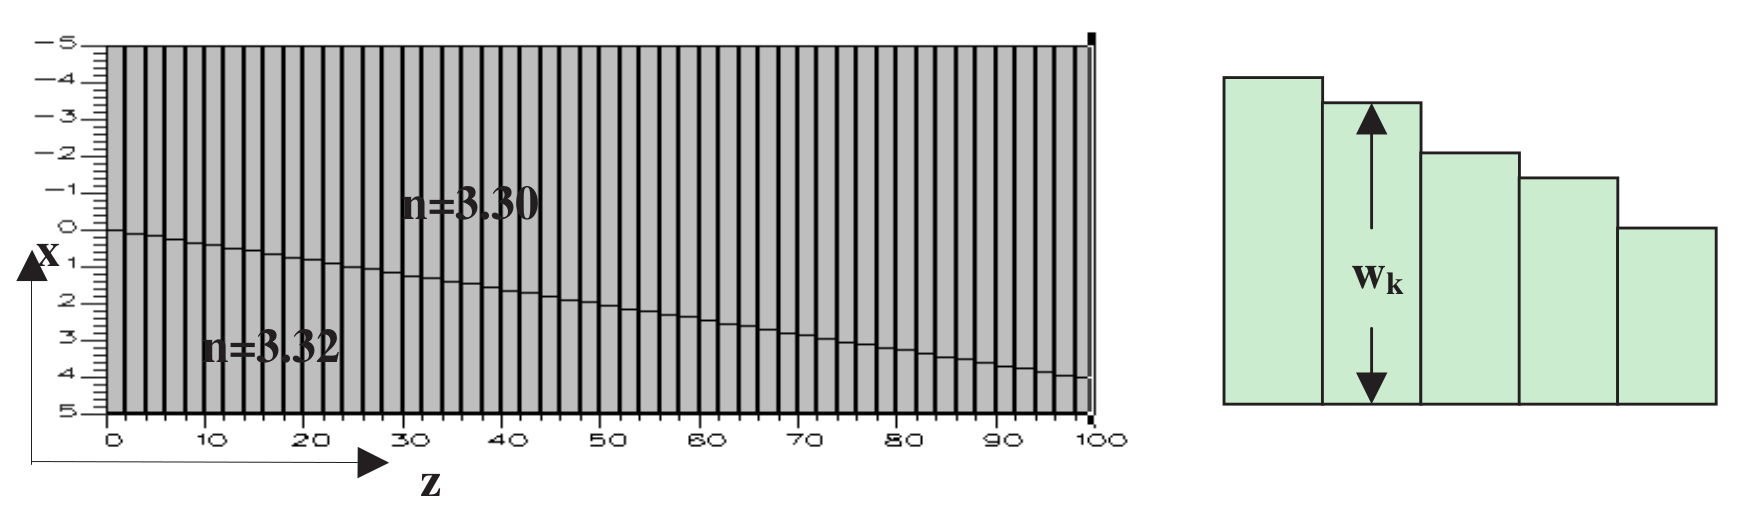
\includegraphics[scale=0.25]{images/numOpti.png}
	\caption{Profil du taper : discrétisation pour le problème d'optimisation}
	\label{fig:numOpti}
\end{figure}

\bigskip
Cette discrétisation impose une régularité très faible pour le profil du taper. On pourrait en effet obtenir des solution avec un profil totalement discontinu. Le champ est calculé grâce à l'analyse faite sur les modes locaux. Les guides d'onde en entrée et en sortie sont choisis tels qu'ils aient au moins un mode guidé. Les dérivées requises sont calculées via un schmé de type différences finies, avec $N=13$ ou $48$ et une solution initiale qui est une droite comme montrée figure \ref{fig:numOpti}.

\subsection{Résultats et interprétation physique}
Les résultats sont assez étonnants : en effet, on pense en général que le profil devrait plutôt ressembler à une courbe assez lisse. Cependant, comme on peut le voir figure \ref{fig:result48}, le résultat n'est pas vraiment ce à quoi on s'attendait. 
\begin{figure}[!h]
	\centering
	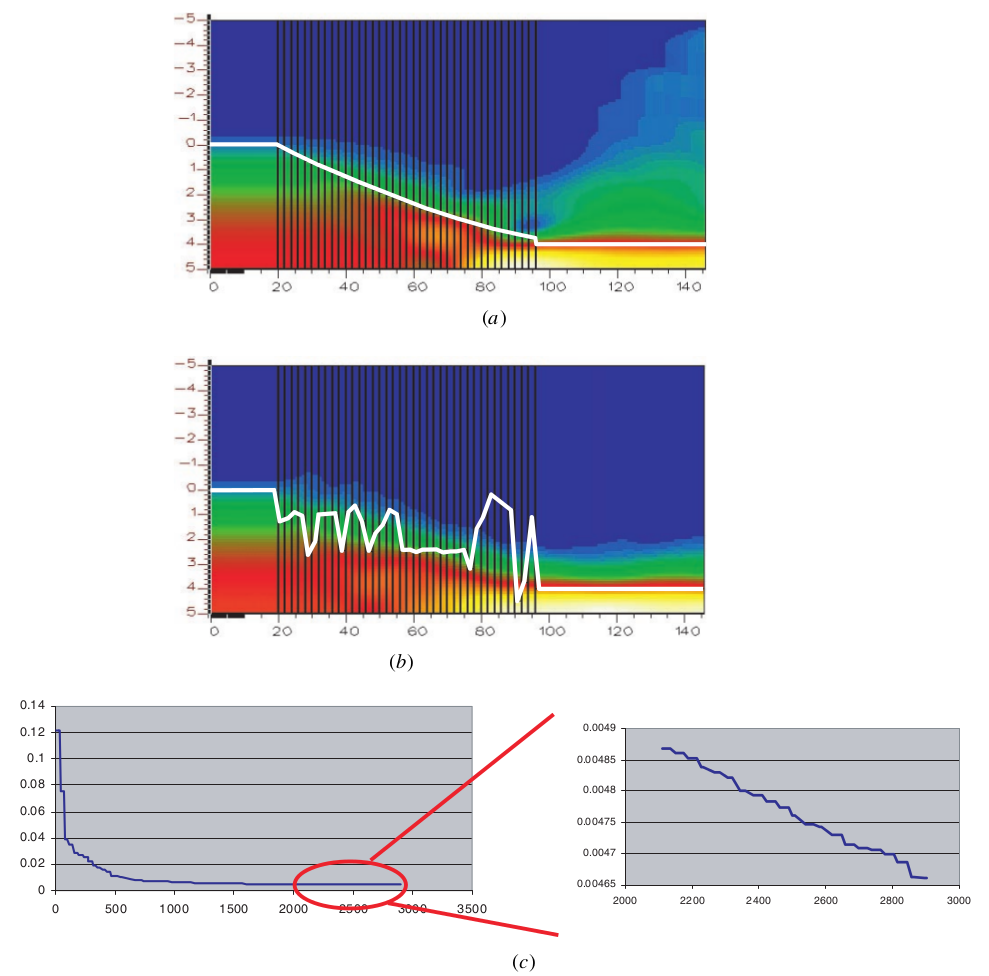
\includegraphics[scale=0.25]{images/result48.png}
	\caption{Profil du taper : résultat avec $N=48$. (a) Forme initial du taper (b) Forme optimale (c) Perte d'énergie en fonction du nombre d'itérations.}
	\label{fig:result48}
\end{figure}
Ces résultats ont été obtenus en 2900 itérations.\\
On remarque dans la figure \ref{fig:powMode} que le mécanisme d'optimisation repose surtout sur une résonnance entre les modes.
\begin{figure}[!h]
	\centering
	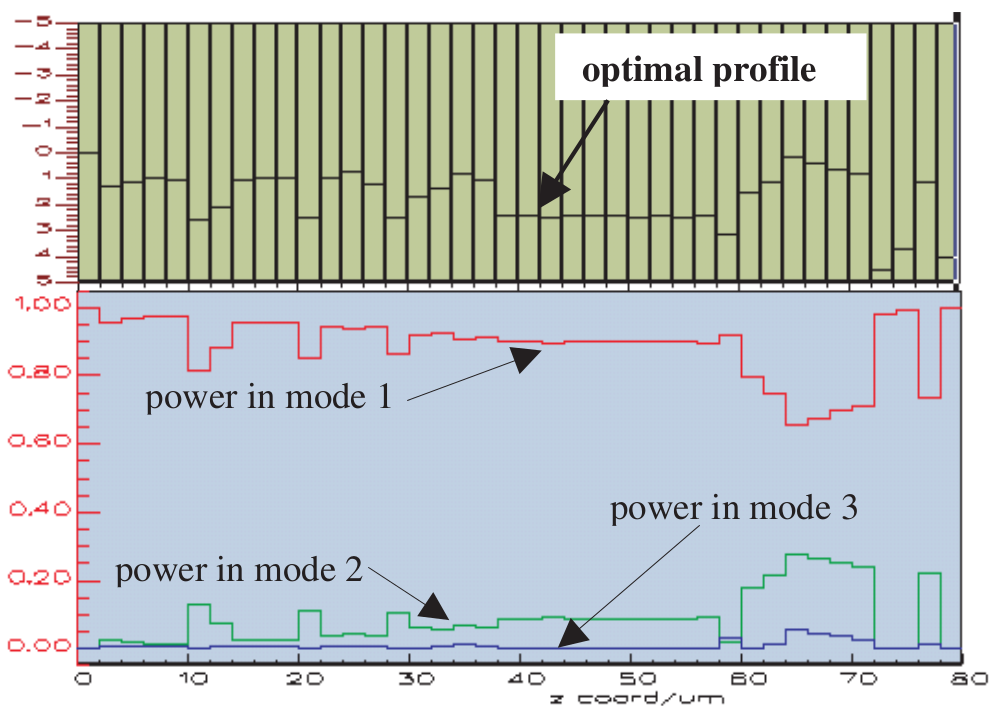
\includegraphics[scale=0.25]{images/powMode.png}
	\caption{L'énergie est préservée grâce à la resonnance avec les autres modes}
	\label{fig:powMode}
\end{figure}
On remarque que le profil est fait de petits pics qui se répètent tous les $10µm$. Cela fait que l'énergie reste presque entièrement dans les deux premiers modes. Après un passage assez plat, le saut final juste avant la fin réintroduit toute la puissance du mode 2 dans le mode 1. La perte d'énergie totale est de seulement 0.5\% en 80µm, tandis qu'un taper plus classique aurait besoin, pour avoir la même efficacité, d'être au moins 5 fois plus long.\\
On ne sait pas, bien sûr, si c'est la solution optimale, mais cette perte d'énergie faible est bien plus importante.\\
Cependant, ces résultats soulèvent une autre problématique : le problème est mal posé.

\subsection{Un problème mal posé}

\bibliographystyle{plain}
\bibliography{bibliographie}
\end{document}
